\documentclass[10pt, a4paper]{article}
\usepackage[latin1]{inputenc}
\usepackage{amsmath}
\usepackage{amsfonts}
\usepackage{amssymb}
\usepackage{graphicx}
\usepackage{xcolor}
\usepackage{float}
\usepackage{hyperref}
\usepackage{booktabs}
\usepackage[normalem]{ulem}
\usepackage{cite}

\usepackage{xcolor}
\hypersetup{
    colorlinks,
    linkcolor={red!50!black},
    citecolor={blue!50!black},
    urlcolor={blue!80!black}
}

% Forcequit autonumbering
\pagenumbering{gobble}


%% Multicolumns
\usepackage{multicol}
\setlength{\columnsep}{1cm}


% Margin to left and middle
\usepackage[margin={2cm,1cm}]{geometry}


\title{Immaterialist Fashion - Report}

\author{Mick van Hulst \and Dennis Verheijden \and Roel van der burg \and Brian Westerweel \and Joost Besseling}

\begin{document}
	\maketitle
	
	
	%% Start multicolumns
	\begin{multicols}{2}
	
	    \section{Introduction}
	    This report describes the results for the first competition of the course Machine Learning in Practice. The source code for this project can be found by going to \href{https://github.com/mickvanhulst/imaterialist_kaggle}{the public Github repository}.
	    \\
	    \\
	    During the project each of the team members were assigned specific tasks. Do take note that our approach can be considered agile as we switched roles constantly and helped each other out where we could:
	    \begin{itemize}
	        \item \textbf{Mick van Hulst:} Exploratory data analysis, GCP, Batch generator, implementing ResNet
	        \item \textbf{Dennis Verheijen:} Implementing networks, general code cleaning, weight determination
	        \item \textbf{Roel van der Burg:} Exploratory data analysis, implementing ResNet
	        \item \textbf{Brian Westerweel:} Implementing custom F1-measure, Object-detection, Report
	        \item \textbf{Joost Besseling:} Object-detection, Ensemble algorithm
	    \end{itemize}
		
		\section{Problem statement}
		We have chosen \href{https://www.kaggle.com/c/imaterialist-challenge-fashion-2018}{the immaterialist fashion challenge} on Kaggle. This challenge consisted of a data set of approximately 1.1 million images which had to be assigned one or multiple labels. In total there are 228 labels that could be assigned of which most don't make sense for the human mind.
		
		
		\section{Data set}
		Kaggle provided a training, validation and test set, combined they consist of approximately 1.1 million images. For each image there is a list containing one or more labels. As mentioned earlier for most of the labels it is unclear why images have a certain label (figure \ref{fig:label_24_examples}). 
		\\
		\begin{figure}[H]
            \centering
            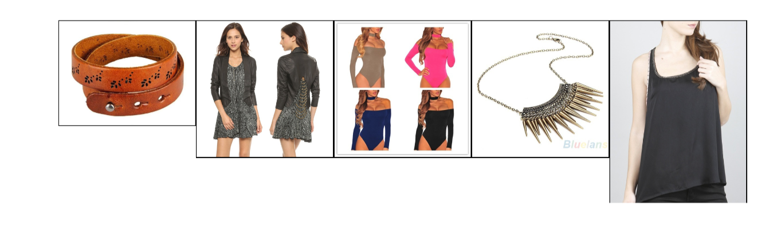
\includegraphics[scale=.4]{img/label24_examples.png}
            \caption{Example images for label 24.}
            \label{fig:label_24_examples}
        \end{figure}
        
        When looking at the individual images label 24 could either be a shirt, necklace, skirt or bracelet. However, apparently there is a more general feature in this images that is represented by label 24 which we couldn't think of.
		
		Another important characteristic of this data set is that it is quite imbalanced (figure \ref{fig:data_dist}). There are around 20 labels which occur more than a 100.000 times each while most of the other labels have roughly 30.000 occurrences.
		\\
		\begin{figure}[H]
            \centering
            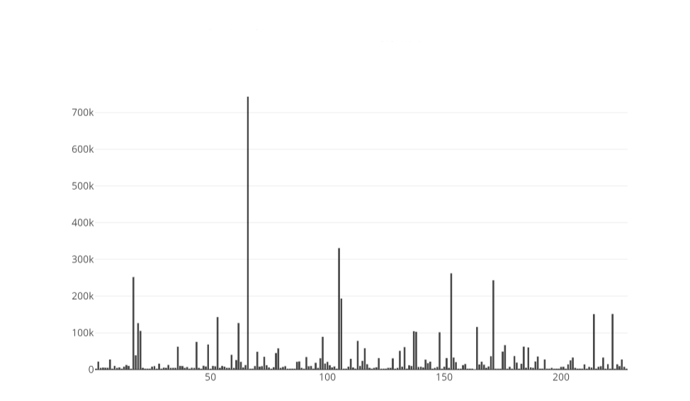
\includegraphics[scale=.4]{img/data_distribution.png}
            \caption{Data distribution, each value on the x-axis representing the label and on the y-axis are the occurences for the labels.}
            \label{fig:data_dist}
        \end{figure}
        The imbalance in the data set posed the challenge of properly training our network by making sure that it doesn't label all images with the most occurring label. This can, for example, be done by setting weights to the different classes so incorrectly labeling a rare label is more heavily penalized than incorrectly labeling a very common label.
	
		\subsection*{Data Preprocessing}
		The data for this challenge didn't need a lot of sanitizing. However, the images were of different sizes and because convolutional neural networks need a static input size we needed to make sure that all images that were fed to the network had the same size. This is accomplished by implementing a patch generator that cut same-sized patches from the source images. 
		
		It has to be noted that due to the gigantic disc size that was needed for the data we decided to download the images at 85\% of the available quality.
		
		\begin{table*}[t]
			\centering
			\begin{tabular}{l|c}
				\toprule
				\textbf{Method} & \textbf{F1-measure (micro-averaged)} \\
				\midrule
				Feature Based Approach v1 & 0.60   \\
				Feature Based Approach v2 & 0.56 \\
				Convolutional Neural Network & 0.49 \\
				Vanilla LSTM & 0.52 \\
				Bidirectional LSTM & 0.93 \\
				\bottomrule
			\end{tabular}
			\caption{Summary of the achieved results, the F1-measure scores are computed using Kaggle.}
			\label{table:summary_results}
		\end{table*}
		
		
		\section{Models}
		During the project multiple approaches have been tried to come up with the final solution. First we implemented an Inception network and trained it on the training set to establish a baseline. After that we trained Inception on a subset of the training data to learn the labels that have more than 100.000 occurrences and on a subset to train the labels that have less than 100.000 occurrences. Besides that, we tried to create a model based on object detected features.
		
		For the loss of all models binary cross entropy is used, because the model has to output a probability for each label. Based on the probability thresholds are determined for each label on when the label actually is there and when not. So after applying the thresholds the output is a list with for the labels associated with an image an '1' and the labels not belonging for that image an '0'.
		
		\subsection{Object detection}
		For the object detection model we first predicted objects for each image using a pre-trained ResNet50 \cite{DBLP:journals/corr/HeZRS15} trained on the open image dataset \cite{openimages}. For each image we used the found objects as features for that image and used those features to train another neurel network. 
		
		However, because the object detection network very often detected just a few objects. Because the object detection network resulted in very small features per image we found very early on that this network would not yield any noteworthy results. Therefore, this model has not been further developed.
		
		\subsection{ResNet50}
		The ResNet we used is based on Keras' version \cite{DBLP:journals/corr/HeZRS15}, where the last layer was unfrozen and fine-tuned to our target data set. 
		
		TODO: MORE EXPLANATION + RESULTS
		
		\subsection{MobileNet}
		MobileNet again is based on a version of Keras \cite{howard2017mobilenets}. In this case the last 5 layers are unfrozen and trained on the training images of this challenge.
		
		TODO: MORE EXPLANATION + RESULTS
		
		\subsection{InceptionV3}
		The InceptionV3 used in this research is based on the pre-trained network from Keras \cite{DBLP:journals/corr/SzegedyVISW15}. Here the last two layers where unfrozen and fine-tuned to the target images.
		
		TODO: MORE EXPLANATION + RESULTS
		
		\section{Ensembling}
		
		TODO: MORE EXPLANATION + RESULTS
	
		\section{Reflection}
		This section briefly discusses some things that stood out during this project.
	    
	\bibliographystyle{unsrt}
	\bibliography{bib}
	\end{multicols}
	
\end{document}